\documentclass[11pt, a4paper]{article}


% Modules essentiels
\usepackage[french]{babel}
\usepackage[T1]{fontenc}
\usepackage[hmargin=2.5cm, vmargin=2.5cm]{geometry}
\usepackage[utf8]{inputenc}
\usepackage[skip=1em]{parskip}


% Modules supplémentaires
\usepackage[algoruled, lined, linesnumbered, longend, french, frenchkw]{algorithm2e}
\DontPrintSemicolon
\SetNlSty{tiny texttt}{}{}

\usepackage{amsfonts}
\usepackage{amsmath}
\usepackage{amssymb}

\usepackage{caption}

\usepackage{color}
\definecolor{mybordeaux}{rgb}{0.43, 0.03, 0.01}
\definecolor{mygray}{rgb}{0.95, 0.95, 0.95}
\definecolor{mygreen}{rgb}{0, 0.6, 0}
\definecolor{myred}{rgb}{0.6, 0, 0}
\definecolor{mypurple}{rgb}{0.73, 0.33, 0.83}

\usepackage{enumitem}
\setlist[itemize]{noitemsep, left=11pt}

\usepackage{graphicx}
\graphicspath{{../images}}

\usepackage{hyperref}
\addto\extrasfrench%
{%
	\def\algorithmautorefname{\textsc{Alg.}}
	\def\equationautorefname{\textsc{Éq.}}
	\def\figureautorefname{\textsc{Fig.}}
	\def\lstlistingautorefname{\textsc{List.}}
	\def\sectionautorefname{\textsc{Sec.}}
	\def\subsectionautorefname{\textsc{Sec.}}
	\def\subsubsectionautorefname{\textsc{Sec.}}
	\def\tableautorefname{\textsc{Tab.}}%
}
\pdfstringdefDisableCommands%
{%
	\def\ce#1{#1}%
}

\usepackage{listings}
\lstset%
{%
	basicstyle=\ttfamily,
	backgroundcolor=\color{mygray},
	breaklines=true,
	captionpos=b,
	commentstyle=\color{mygreen},
	emphstyle=\color{mybordeaux},
	extendedchars=true,
	firstnumber=1,
	frame=single,
	keywordstyle=\color{myred},
	language=Python,
	literate= {À}{{\`A}}1 {à}{{\`a}}1 {é}{{\'e}}1 {è}{{\`e}}1,
	numbers=left,
	numberstyle=\tiny\color{black},
	showstringspaces=true,
	stepnumber=5,
	stringstyle=\color{mypurple},
	tabsize=3%
}

\usepackage[version=4]{mhchem}

\usepackage[space-before-unit, per-mode=power, inter-unit-product=.]{siunitx}

\usepackage{subcaption}

\usepackage{tabularx}

\usepackage{xfrac}


% Caractéristiques du document
\title{Construction de configurations intitiales}
\author{Heiarii Lou Chao}
%\date{}


\begin{document}
\maketitle
%\tableofcontents

\section{Introduction}

Nous voulons construire une configuration initiale d'une structure constituée de deux plaques (ou couches) de graphite séparées l'une de l'autre par de l'eau.

Pour cela, nous utilisons les outils : \href{https://jp-minerals.org/vesta/en/}{VESTA} et \href{https://m3g.github.io/packmol/index.html}{PACKMOL}, respectivement pour la visualisation et la construction des molécules et pour l'optimisation de leur répartition.

\section{Présentation de la structure}

La structure est représentée à la \autoref{fig:structure}, avec les couches de graphite en gris et l'eau en bleu.

\begin{figure}[hpbt]
	\centering
	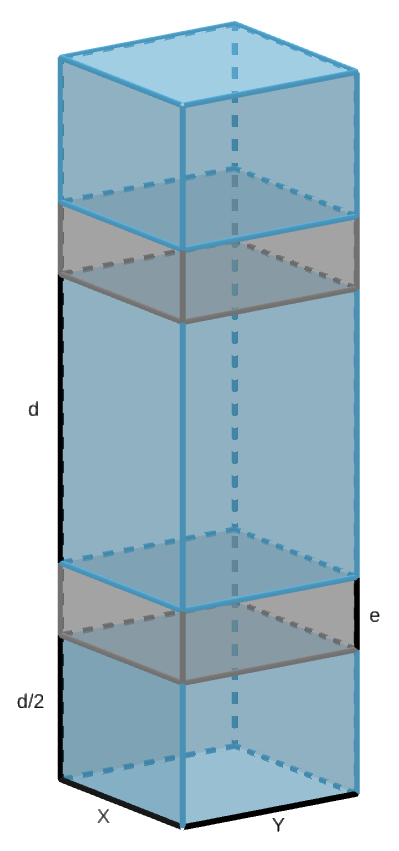
\includegraphics[scale=0.3]{structure.png}
	\caption{Structure à construire}
	\label{fig:structure}
\end{figure}

\section{Déroulement de la construction}

Le déroulement des étapes pour la construction des structures cristallines est présenté à la \autoref{fig:deroulement}.

\begin{figure}[hpbt]
	\centering
	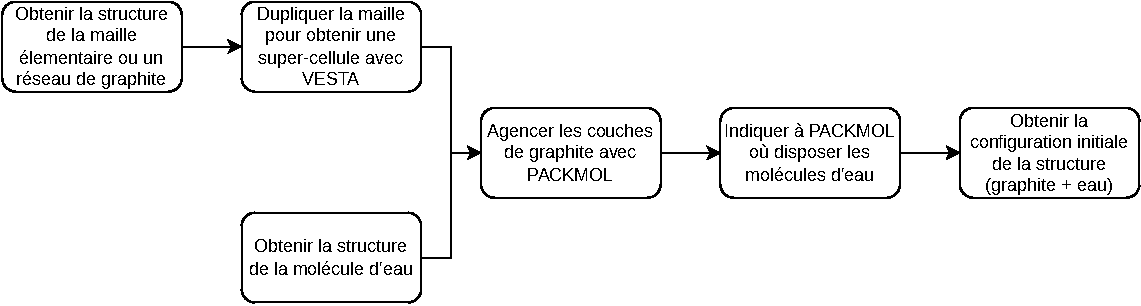
\includegraphics[width=\linewidth]{construction-deroulement.pdf}
	\caption{Étapes de la construction des configurations initiales}
	\label{fig:deroulement}
\end{figure}

Les données sur les structures des molécules ont été obtenu grâce à la \href{http://www.crystallography.net/cod/}{Crystallography Open Database} (COD), celles-ci sont présentées à la \autoref{fig:molecules_initiales}.

\begin{figure}[hpbt]
	\centering
	\begin{subfigure}{\linewidth}
		\centering
		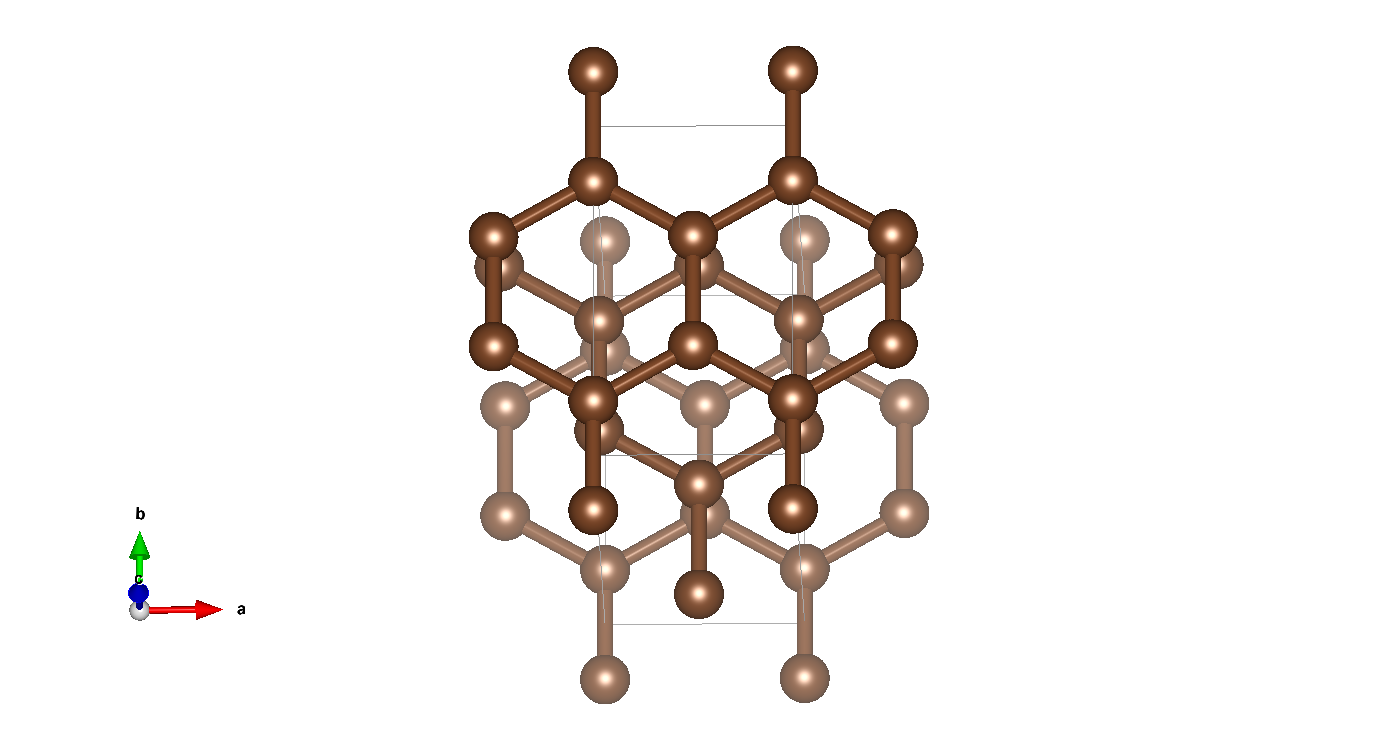
\includegraphics[scale=0.2]{graphite.png}
		\caption{Réseau de graphite}
	\end{subfigure}
	\begin{subfigure}{\linewidth}
		\centering
		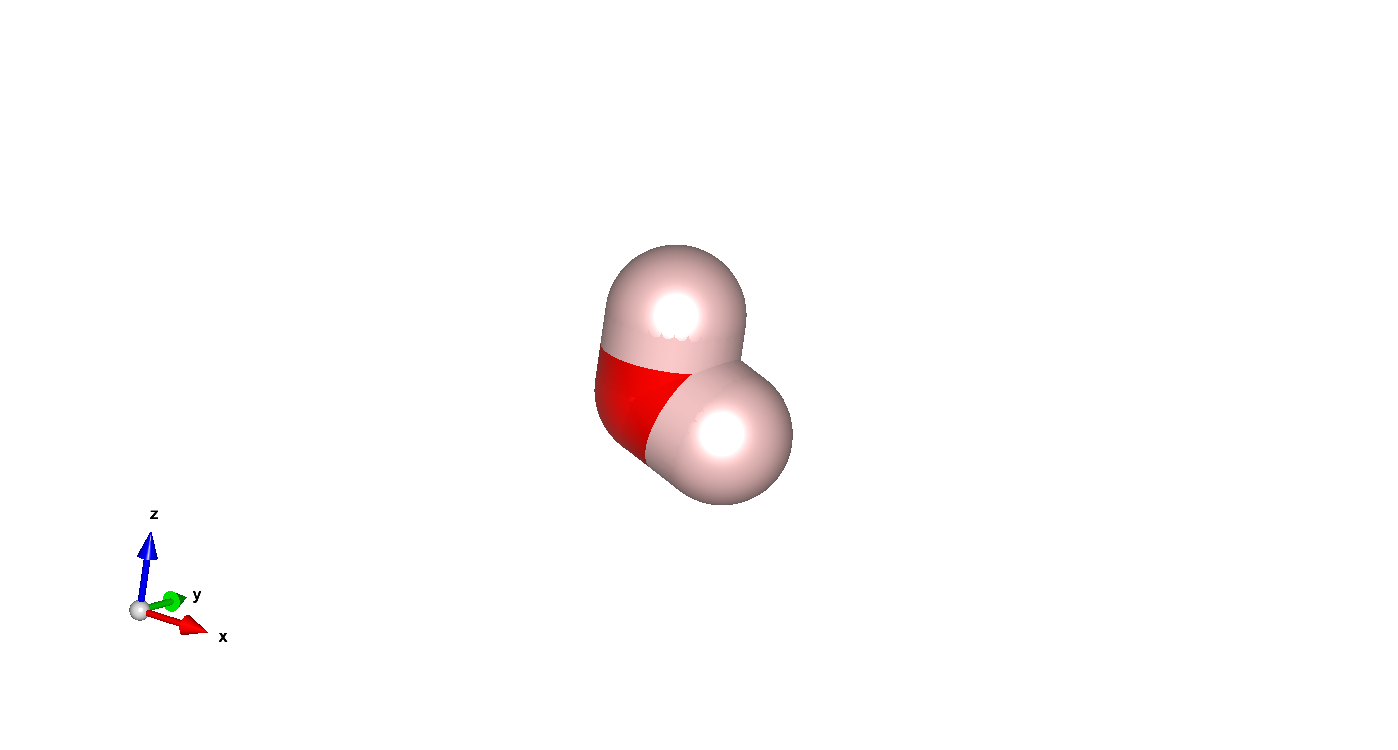
\includegraphics[scale=0.2]{water.png}
		\caption{Molécule d'eau}
	\end{subfigure}
	\caption{Structures des molécules provenant de la COD}
	\label{fig:molecules_initiales}
\end{figure}

	\subsection{Construction de la super-cellule}

		\subsubsection{Taille de la super-cellule}

Nous avons obtenu un réseau de graphite, et non la maille élémentaire, celui-ci est dupliqué quatre fois dans les directions $[Ox)$ et $[Oy)$ pour construire une couche/plaque de graphite, ainsi nous avons :
\begin{align*}
	X &= \num{4} \times a\\
	Y &= \num{4} \times b\\
	e &= c\\
\end{align*}
où $a$, $b$ et $c$ sont la longueur, la largeur et la hauteur du réseau.

		\subsubsection{Conditions aux limites périodiques}

Pour que les atomes situés aux bords ne se chevauchent pas lorsque l'on appliquera les conditions aux limites, il est nécessaire de :
\begin{itemize}
	\item supprimer une option : \lstinline!Edit > Bonds > Boundary mode > Do not search atoms beyond the boundary!
	\item définir l'amplitude des coordonnées fractionnaires (pour la duplication) non entières, dans notre cas on veut dupliquer le réseau initial \num{4} fois, alors met : \lstinline!Objects > Boundary > Ranges of fractional coordinates > x(max) = 3.99, y(max) = 3.99!
\end{itemize}

	\subsection{Agencement des couches de graphite}

Nous indiquons à PACKMOL de disposer les couches de graphite de la manière suivante :
\begin{itemize}
	\item la couche inférieure a son centre fixé en $(\frac{X}{2}, \frac{Y}{2}, \frac{d}{2} + \frac{e}{2})$
	\item la couche supérieure a son centre fixé en $(\frac{X}{2}, \frac{Y}{2}, \frac{3 \times d}{2} + \frac{3 \times e}{2})$
\end{itemize}

	\subsection{Disposition des molécules d'eau}

Pour disposer les molécules d'eau, l'outil a besoin -- en plus de la structure de la molécule d'eau -- de la distance minimale entre les molécules (la tolérance, notée $tol$), du nombre de molécules et des limites des régions où placer les molécules.

		\subsubsection{Distance entre les molécules}

La distance minimale entre les molécules est obtenue en étudiant la fonction de corrélation de paires de l'eau à l'état liquide, présentée à la \autoref{fig:RDF_eau}.

Nous pouvons en déduire l'agencement des molécules d'eau du liquide :
\begin{itemize}
	\item Le premier pic de $g_{\ce{OH}}$ correspond à la distance des liaisons \ce{O-H} d'une molécule d'eau
	\item Le second pic de $g_{\ce{OH}}$ correspond à la distance des liaisons hydrogène \ce{H-O}
	\item Le troisième pic de $g_{\ce{OH}}$ correspond à la distance entre un atome d'\ce{O} d'une molécule à un atome d'\ce{H} d'une autre molécule d'eau
	\item Le premier pic de $g_{\ce{HH}}$ correspond à la distance entre deux atomes d'\ce{H} d'une même molécule
	\item Le premier pic de $g_{\ce{OO}}$ correspond à la distance entre deux atomes d'\ce{O} de deux molécules
\end{itemize}

Les pics pertinents pour notre problème sont : le second pic de $g_{\ce{OH}}$ et le premier pic de $g_{\ce{OO}}$ car ils caractérisent des distances entre les molécules d'eau.\\
Finalement, nous choisissons une \fbox{tolérance de \qty{1.5}{\angstrom}} correspondant au début du second pic de $g_{\ce{OH}}$ pour deux raisons :
\begin{itemize}
	\item cela permet à PACKMOL de converger plus facilement
	\item on obtient un système réaliste puisque des liaisons hydrogène sont permises
\end{itemize}

\begin{figure}[hptb]
	\centering
	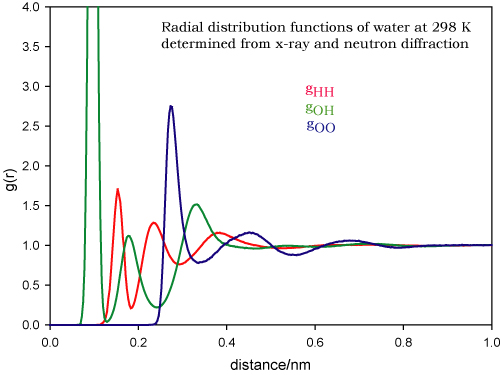
\includegraphics[width=\linewidth]{RDF_eau.jpg}
	\caption{Fonctions de corrélation de paires de l'eau (\url{http://rkt.chem.ox.ac.uk/lectures/liqsolns/liquids.html})}
	\label{fig:RDF_eau}
\end{figure}

		\subsubsection{Nombre de molécules}

Nous pouvons calculer le nombre de molécules d'eau avec la formule suivante :
	\[ N = \frac{\rho V \mathcal{N}_A}{M} \]
avec $\rho$ la masse volumique, $V$ le volume, $\mathcal{N}_A$ le nombre d'Avogadro et $M$ la masse molaire.

Nous prenons $\rho_{H_2O} = \qty{1.000e+03}{\kg \per \cubic\m}$, $\mathcal{N}_A = \qty{6.022e+23}{\per \mol}$ et $M_{H_2O} = \qty{1.801e-02}{\kg \per \mol}$.

Alors, avec les dimensions du réseau initial,
\begin{equation*}
	\left\lbrace
	\begin{aligned}
		a &= \qty{2.456e-10}{\m}\\
		b &= \qty{4.254e-10}{\m}\\
		c &= \qty{6.696e-10}{\m}
	\end{aligned}
	\right.
\end{equation*}
et en prenant $d = \qty{20.00e-10}{\m}$, les volumes sont :
\begin{align*}
	V_1 &\approx \qty{1672e-30}{\cubic \m}\\
	V_2 &\approx \qty{3344e-30}{\cubic \m}
\end{align*}
où $V_1$ est le volume des régions inférieure et supérieure et $V_2$ est le volume de la région centrale.

Finalement, les nombres de molécules d'eau à placer sont :
\begin{equation*}
	\boxed%
	{
	\begin{aligned}
		N_1 &\approx \num{56}\\
		N_2 &\approx \num{112}
	\end{aligned}
	}
\end{equation*}

		\subsubsection{Limites des régions et conditions aux limites périodiques}

Pour que des molécules d'eau ne se chevauchent pas une fois que nous appliquerons les conditions aux limites périodiques, il est conseillé (\href{https://m3g.github.io/packmol/userguide.shtml#pbc}{manuel de PACKMOL}) de réduire la taille de la boîte : en minimisant l'énergie, les molécules d'eau se répartiront dans l'espace dont elle disposerons.\\
Nous réduisons les dimensions de la boîte (aux extrémités, dans les trois directions de l'espace) de la moitié de la tolérance, c'est-à-dire de \qty{0.750}{\angstrom}.

Les trois régions de l'espace où doivent être disposées les molécules d'eau sont alors données par :
\begin{itemize}
	\item une boîte délimitée par $(\frac{tol}{2}, \frac{tol}{2}, \frac{tol}{2})$ et $(X - \frac{tol}{2}, Y - \frac{tol}{2}, \frac{d}{2})$
	\item une autre délimitée par $(\frac{tol}{2}, \frac{tol}{2}, \frac{d}{2} + e)$ et $(X - \frac{tol}{2}, Y - \frac{tol}{2}, \frac{3 \times d}{2} + e)$
	\item une dernière délimitée par $(\frac{tol}{2}, \frac{tol}{2}, \frac{3 \times d}{2} + 2 \times e)$ et $(X - \frac{tol}{2}, Y - \frac{tol}{2}, 2 \times d + 2 \times e - \frac{tol}{2})$
\end{itemize}

\section{Configuration initiale obtenue}

Nous obtenons la configuration initiale de la \autoref{fig:configuration_initiale}.

\begin{figure}[hptb]
	\centering
	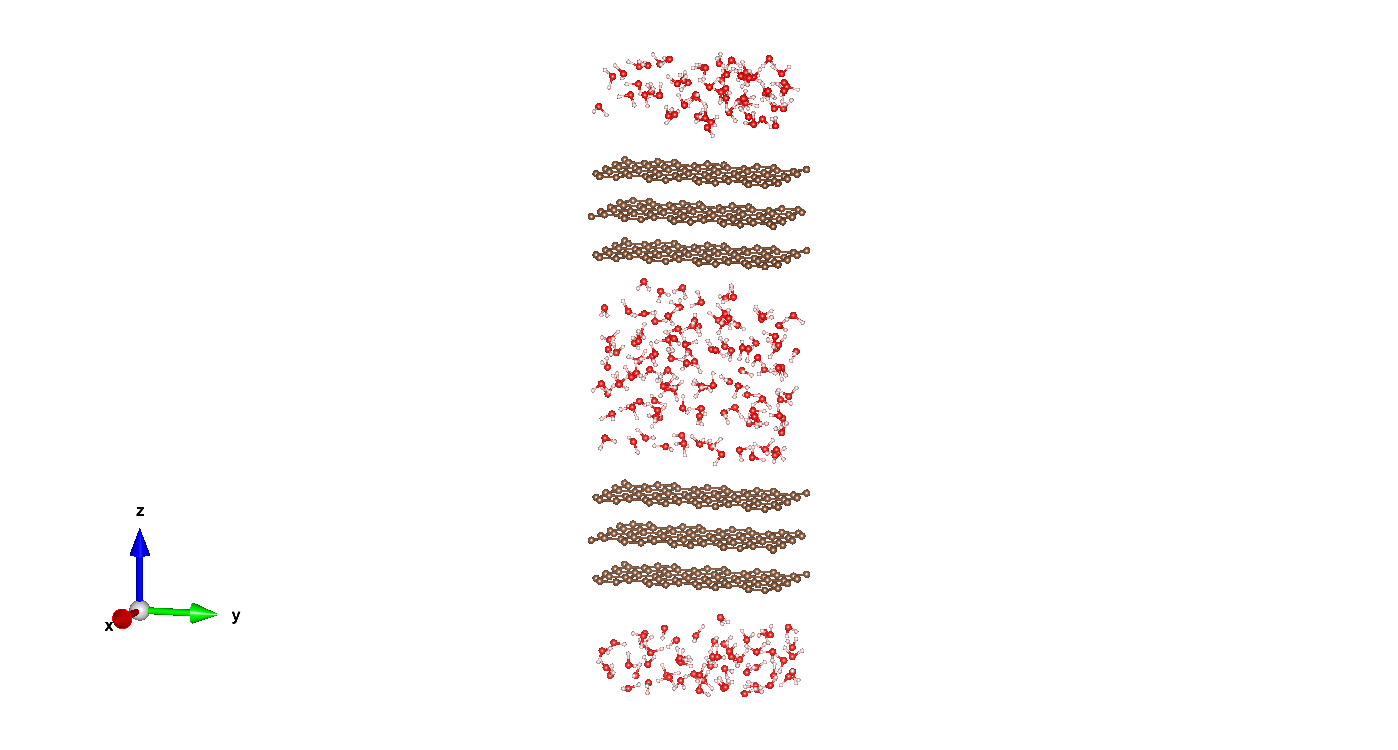
\includegraphics[width=\linewidth]{configuration_initiale.png}
	\caption{La configuration initiale obtenue de la structure (graphite + eau)}
	\label{fig:configuration_initiale}
\end{figure}

\end{document}